

\documentclass[11pt]{article}
\usepackage[utf8]{inputenc}
\usepackage{geometry}
\usepackage{graphicx}
\usepackage{hyperref}
\usepackage{amsmath}
\usepackage{listings}
\usepackage{xcolor}
\usepackage{float}
\usepackage{subcaption}
\usepackage{algorithm}
\usepackage{algpseudocode}
\usepackage{booktabs} % For prettier tables
\usepackage{siunitx}
\usepackage{amssymb}
\usepackage{subcaption}

% Set page margins
\geometry{a4paper, margin=1in}

% Set up code listing style
\lstset{
    basicstyle=\ttfamily,
    commentstyle=\color{gray},
    keywordstyle=\color{blue},
    stringstyle=\color{red},
    showstringspaces=false,
    captionpos=b
}

\title{Image Analysis Coursework}
\author{Vishal Jain}
\date{\today}

\begin{document}
\section{Question 1 - Image Segmentation}
This question details the segmentation algorithms used to segment the required sections of the lung ct image, the noisy flowers and the coin images.
\subsection{Part A: Lung CT Image Segmentation}
This section details the segmentation algorithm of the Lung CT image shown in Figure \ref{fig:lung_ct_image}. The region to be segmented is the lung area, including all the nodules and tissue within. The image is taken from the LIDC-IDRI dataset \cite{lidc_idri}.
\begin{figure}[H]
    \centering
    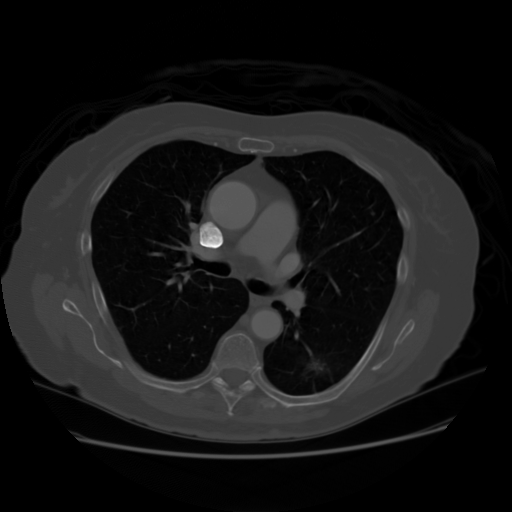
\includegraphics[width=0.5\textwidth]{../data/CT.png}
    \caption{Lung CT image from the LIDC-IDRI dataset.}
    \label{fig:lung_ct_image}
\end{figure}

\subsubsection{Image Characteristics}
The image shows a high contrast between the lungs and surrounding non lung tissue. This observation motivates a threshold based approach to segment the lung area. The nodules and tissue in the intra lung regions are of a much higher intensity than the lung tissue, as such it is appropriate supplement the thresholding step with additional morphological operations.

\subsubsection{Assumptions}
The algorithm assumes that after binarising the image via thresholding, the background makes up the largest connected component, with the left and right lungs being the next two largest. The algorithm also assumes that the nodules and tissue within the lung regions are fully enclosed and do not touch the border of the lung regions.

\subsubsection{Segmentation Algorithm}
The segmentation algorithm for the lung CT image is as follows:
\begin{itemize}
    \item \textbf{Binarise Image via Otsu Thresholding:} The image is thresholded using Otsu's threshold. This is a global thresholding method that maximises the inter-class variance of foreground and background. 
    \item \textbf{Connected Component Analysis:} The binary image is inverted to make the lung and background regions the foreground. The connected components of the inverted image are labelled using 8-connectivity. The second and third largest connected components are selected to recover the left and right lung regions. The connected components are selected based on their area. 
    \item \textbf{Binary Hole Filling} To recover the nodules and tissue within the lung regions, binary hole filling is performed. The algorithm fills holes in a binary image by inverting the image, labelling connected regions, and converting regions not connected to the border from background to foreground.
    \end{itemize}
    \begin{figure}[H]
        \centering
        \begin{subfigure}{.3\textwidth}
            \centering
            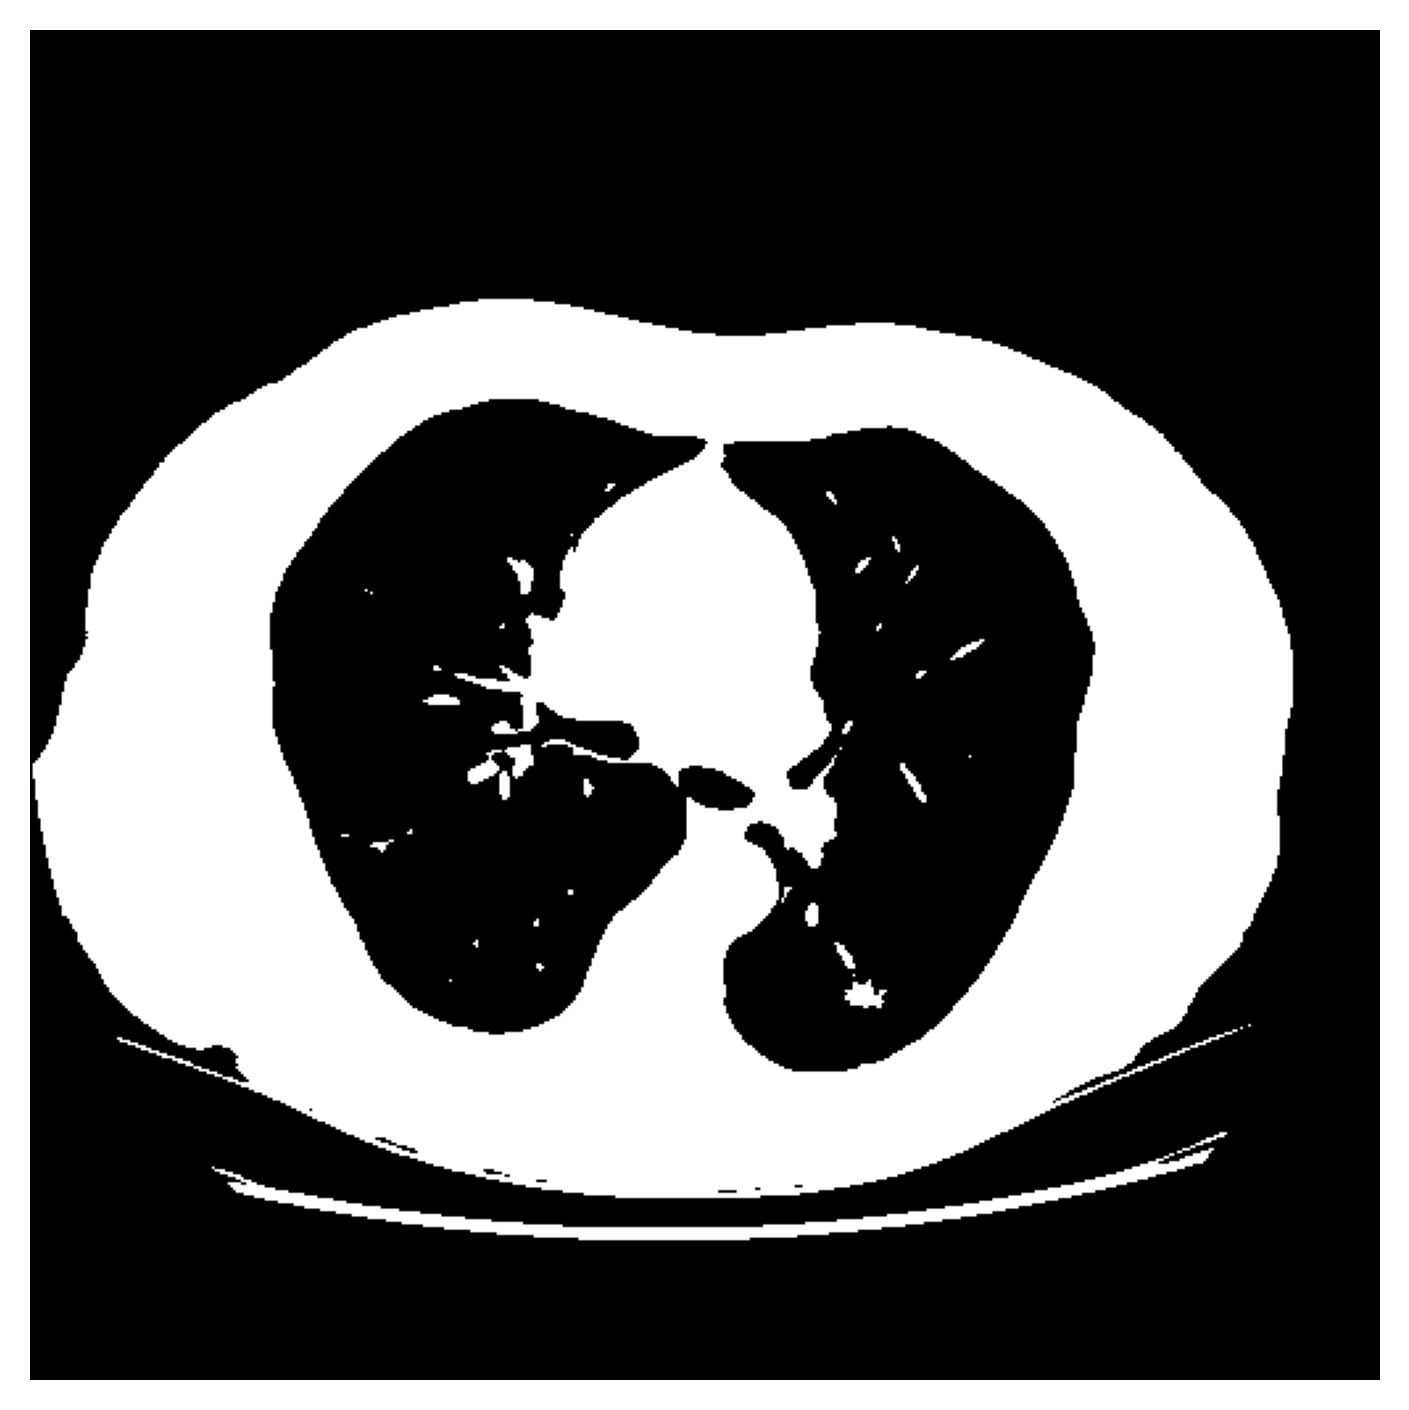
\includegraphics[width=\linewidth]{figs/q1a_binary.png}  % Replace with your image file
            \caption{}
            \label{fig:otsu_threshold}
        \end{subfigure}%
        \begin{subfigure}{.3\textwidth}
            \centering
            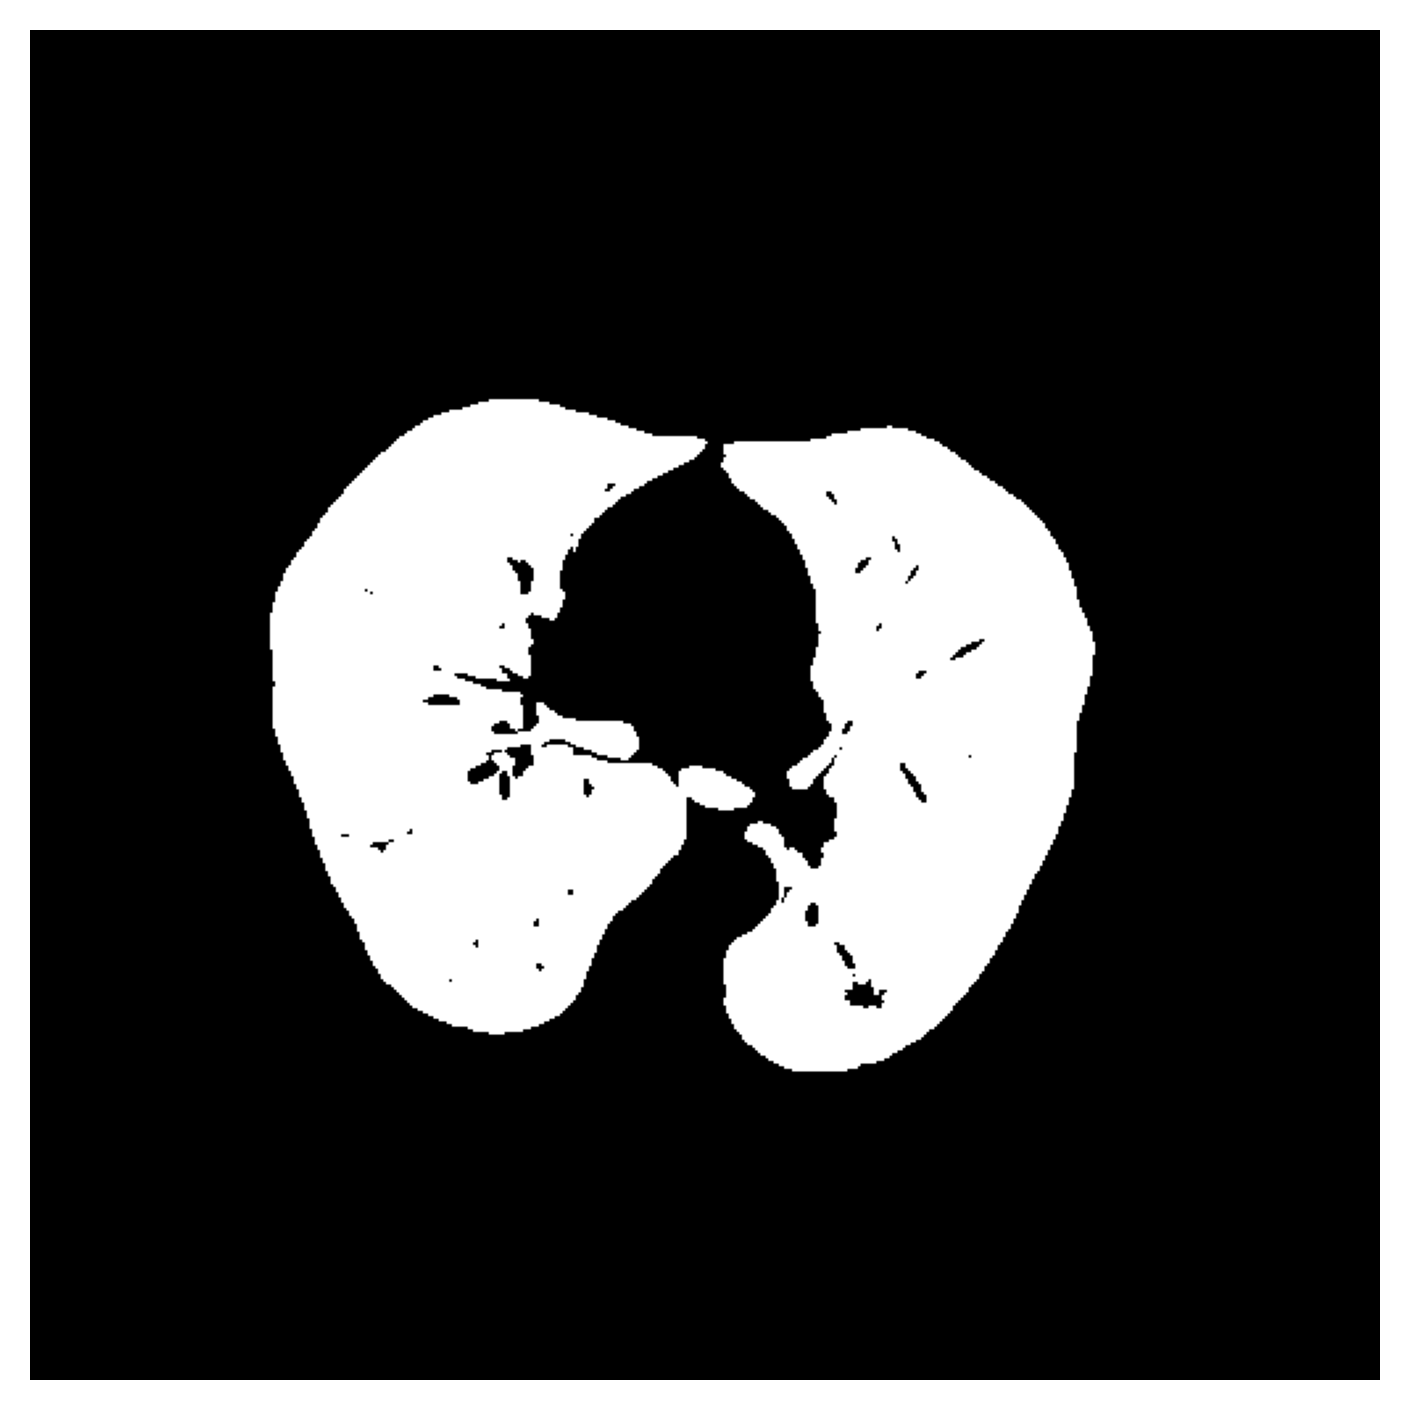
\includegraphics[width=\linewidth]{figs/q1a_largest_connected_components.png}  % Replace with your image file
            \caption{}
            \label{fig:connected_components}
        \end{subfigure}%
        \begin{subfigure}{.3\textwidth}
            \centering
            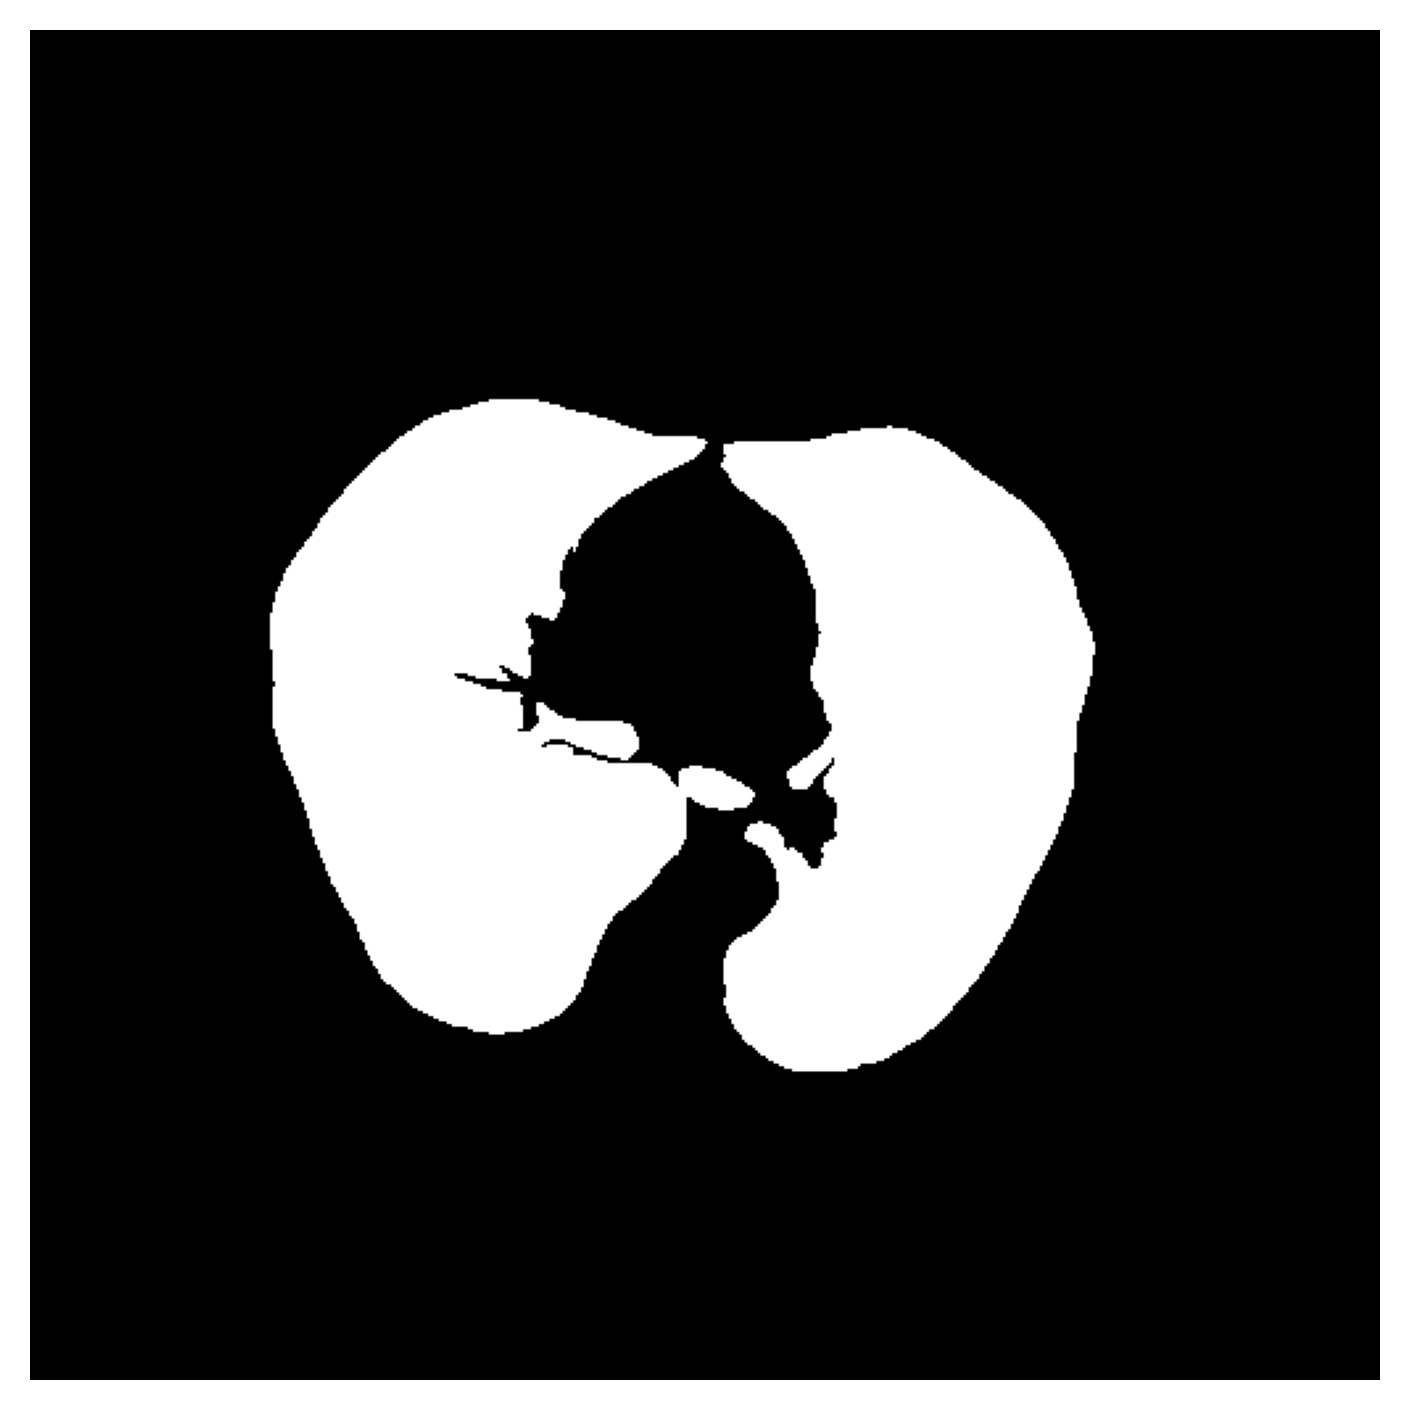
\includegraphics[width=\linewidth]{figs/q1a_filled_holes.png}  % Replace with your image file
            \caption{}
            \label{fig:filled_holes}
        \end{subfigure}
        \label{fig:segmentation_steps}
    \caption{Key steps in the segmentation of the lung CT image: (a) Binarisation using Otsu's threshold, (b) Mask inversion and selection of lung regions via connected component analysis, (c) Recovery of internal structures through binary hole filling.}
    \end{figure}
Note, this segmentation algorithm was also implemented from scratch. Relevant code can be found in \texttt{src/q1a\_from\_scratch.py} and \texttt{src/from\_scratch\_seg\_funcs.py}.
\subsubsection{Results}
The final segmentation of the lung CT image is shown in Figure \ref{fig:lung_ct_image} The segmentation clearly captures the relevant lung regions and all the nodules and tissues within.
\begin{figure}[H]
    \centering
    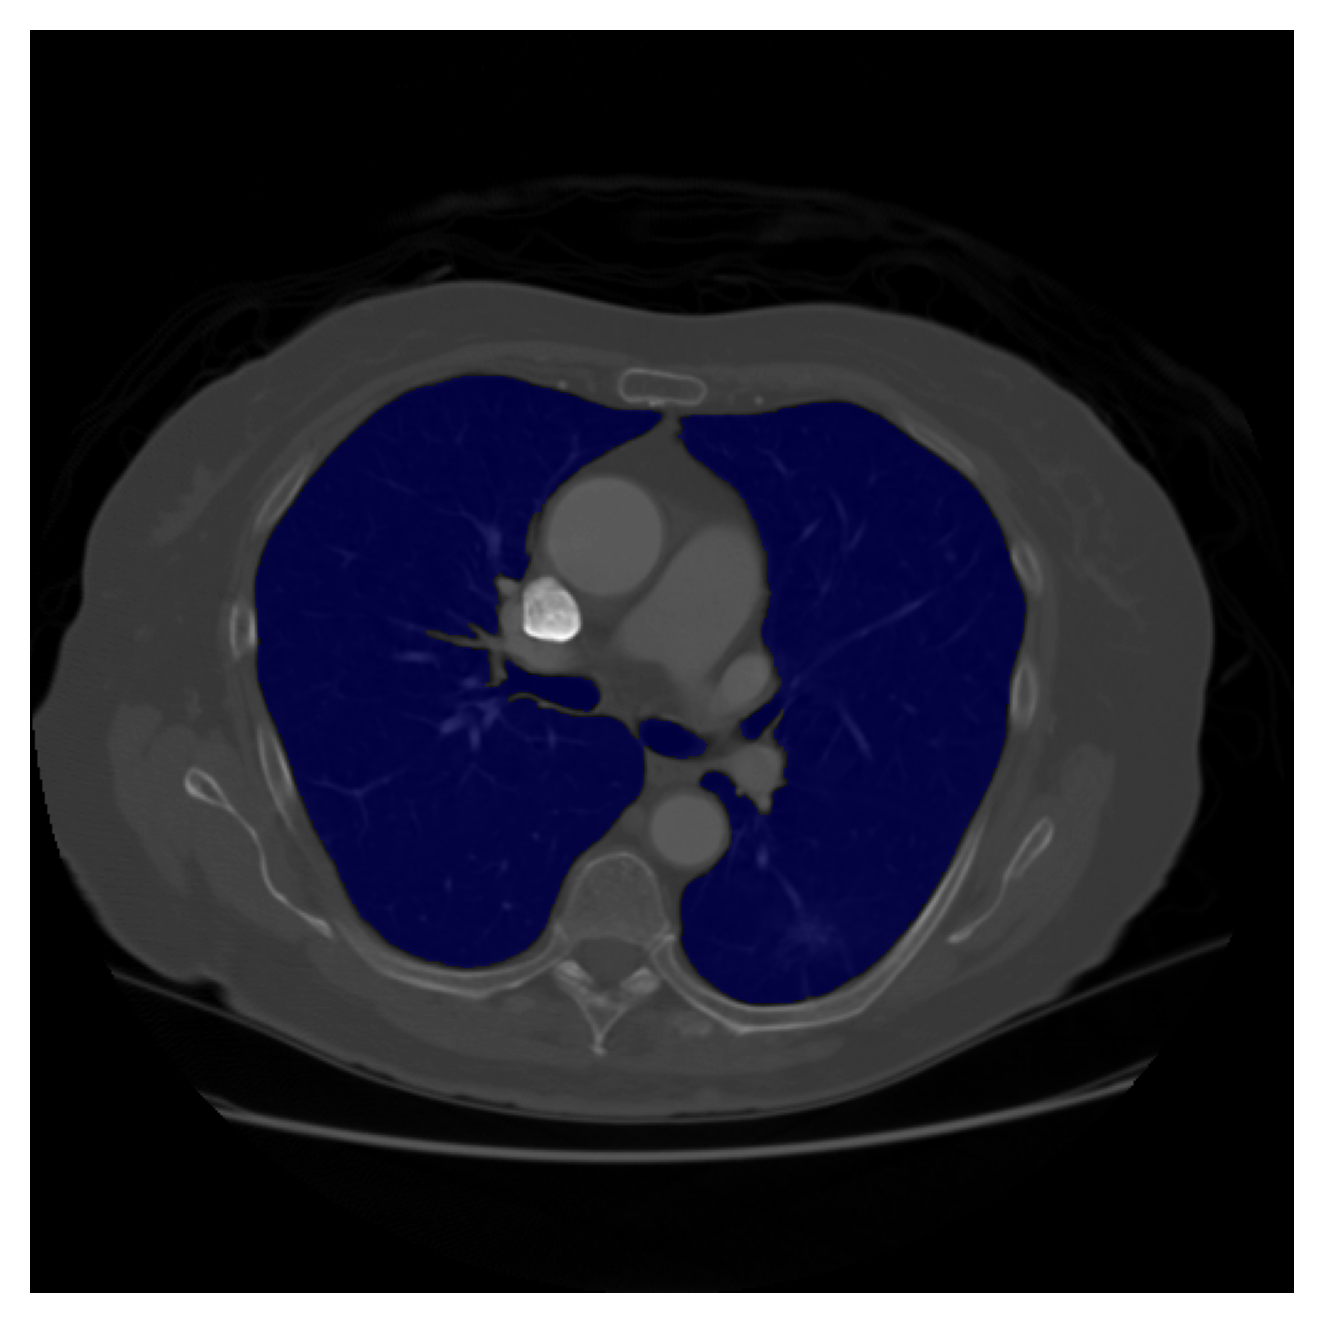
\includegraphics[width=0.4\textwidth]{figs/q1a.png}
    \caption{Final segmentation of the lung CT image.}
    \label{fig:lung_ct_segmentation}
\end{figure}

\subsubsection{Discussion}
Figure \ref{fig:q1a_ambiguity} shows a potential ambiguous region in the segmentation. This region was segmented due to having a similar intensity as the lung tissue and being connected to lung tissue post Otsu thresholding. However, as this region could not be clearly identified as non lung tissue without additional context, it was kept in the final segmentation. This also highlights the limitations of thresholding based segmentation methods in identifying regions that are not clearly defined by intensity.
\begin{figure}[H]
    \centering
    \begin{subfigure}{.4\textwidth}
        \centering
        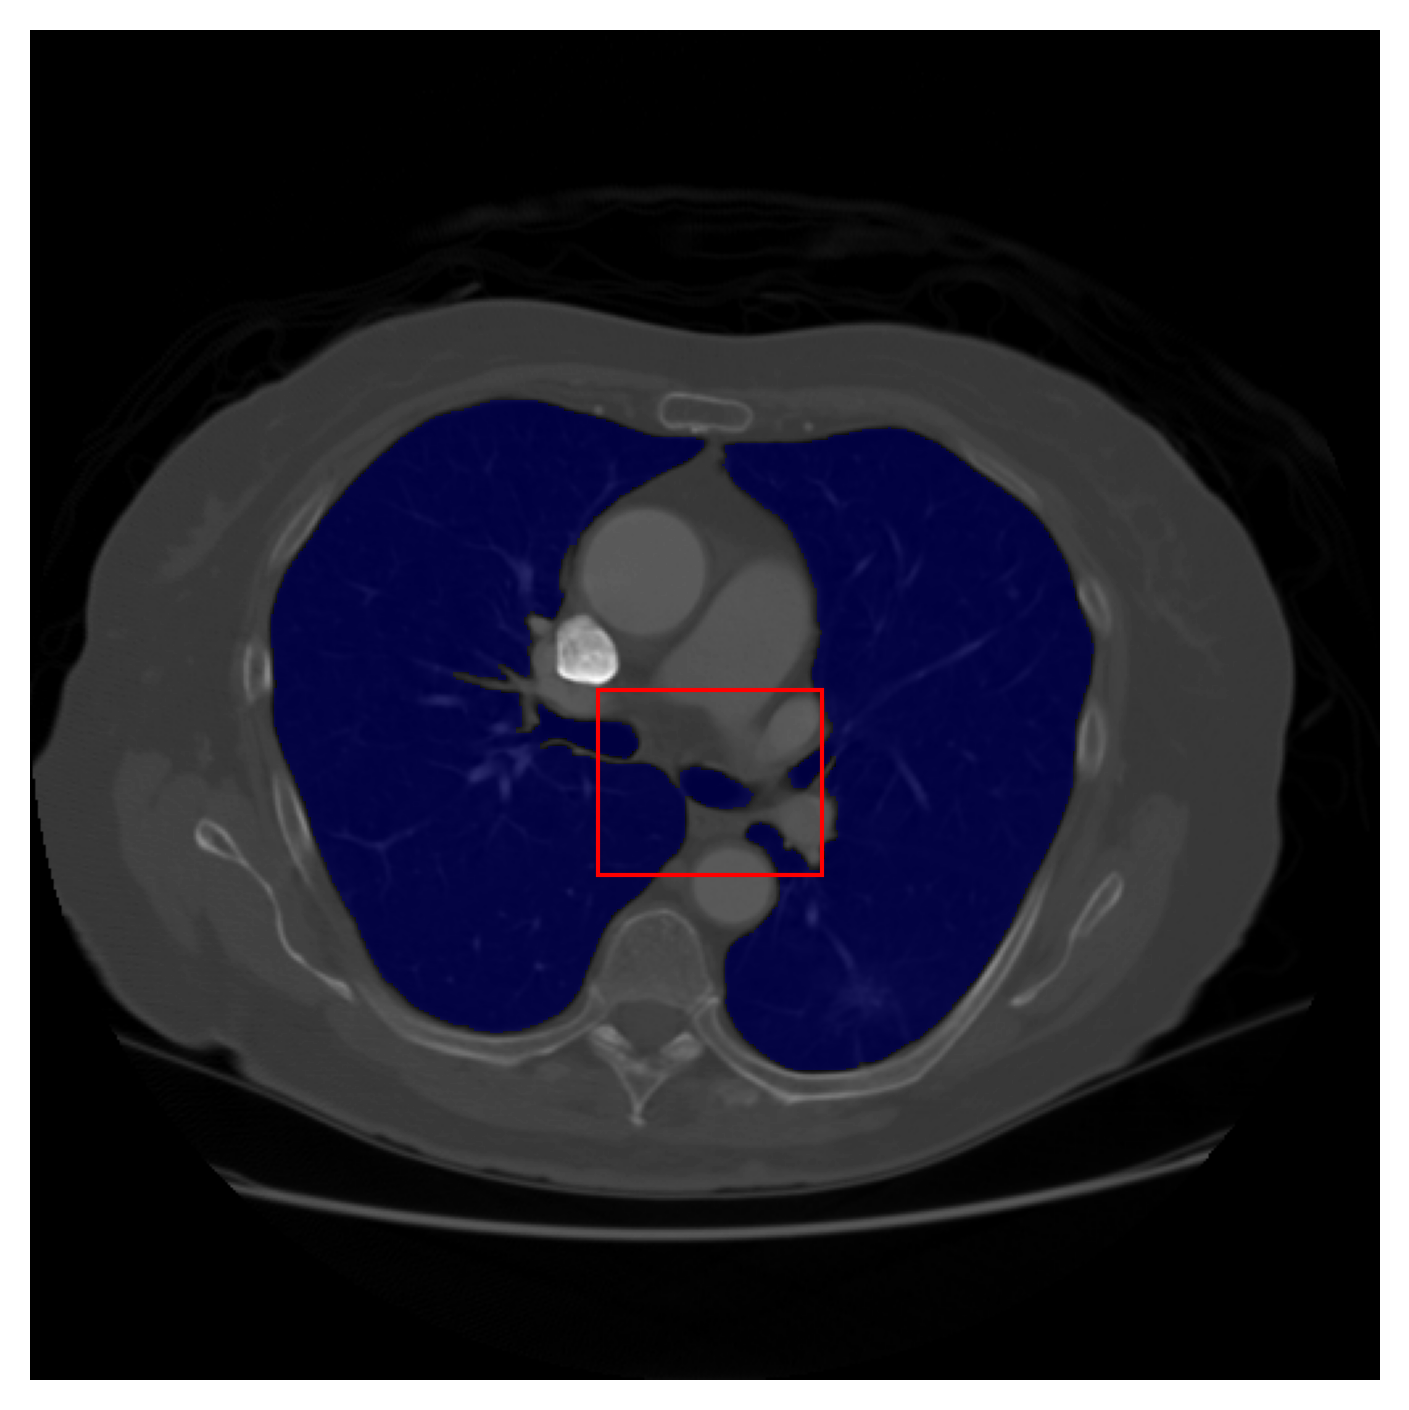
\includegraphics[width=\linewidth]{figs/q1a_seg_w_bbox.png}  % Replace with your image file
        \caption{}
        \label{fig:q1a_seg_w_bbox}
    \end{subfigure}%
    \begin{subfigure}{.4\textwidth}
        \centering
        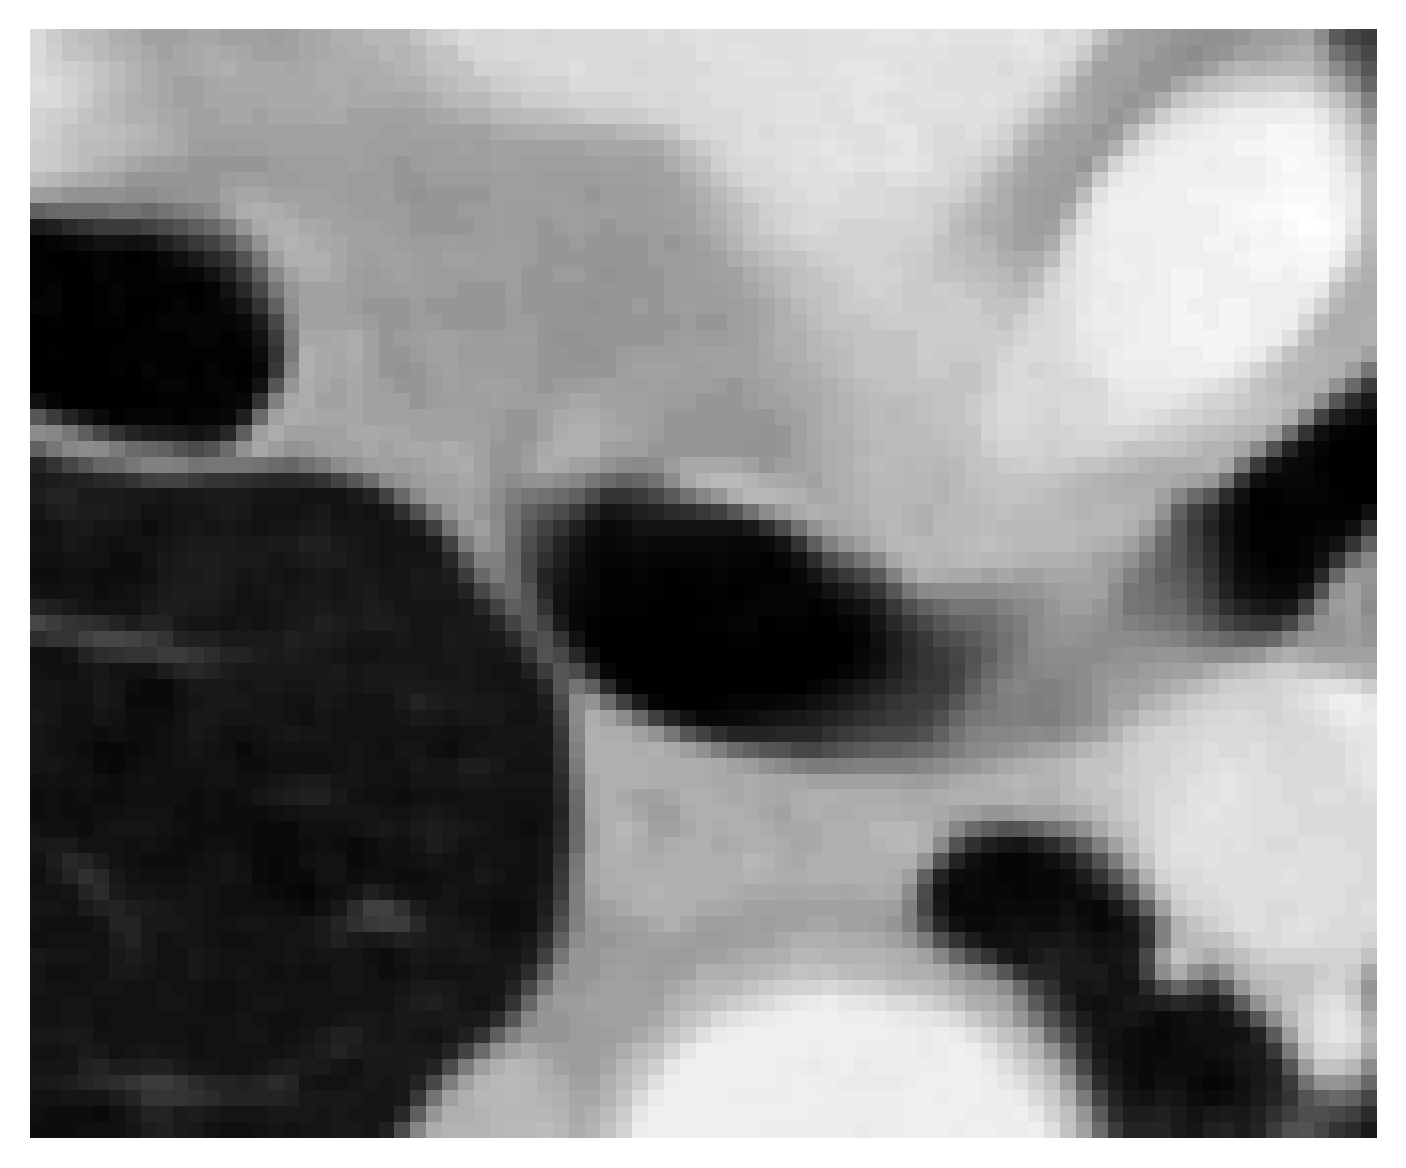
\includegraphics[width=\linewidth]{figs/q1a_zoomed_region.png}  % Replace with your image file
        \caption{}
        \label{fig:q1a_zoomed_region}
    \end{subfigure}%
    \caption{Ambiguous region in the segmentation: (a) Segmentation with bounding box around the ambiguous region, (b) Zoomed in view of the ambiguous region.}
    \label{fig:q1a_ambiguity}
\end{figure}

\subsection{Part B: Noisy Flowers Image Segmentation}
This section details the segmentation algorithm of the noisy flowers image shown in Figure \ref{fig:flowers_image}. The region to be segmented are all the purple flower heads in the image.

\begin{figure}[H]
    \centering
    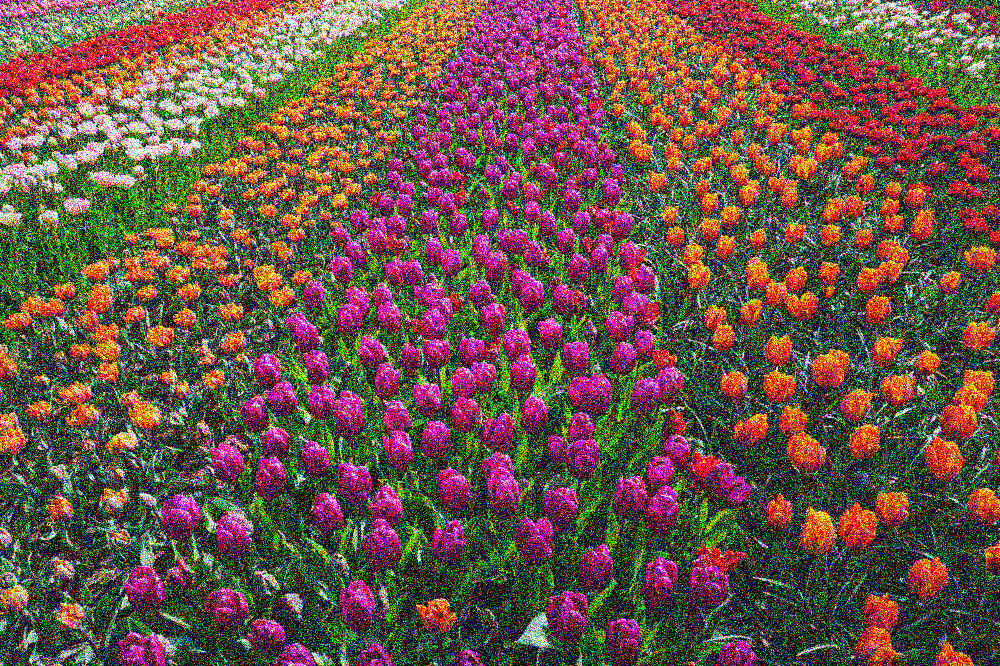
\includegraphics[width=0.8\textwidth]{../data/noisy_flower.jpg}
    \caption{Noisy Flowers image.}
    \label{fig:flowers_image}
\end{figure}

\subsubsection{Image Characteristics}
The image features a type of noise that is typical to gaussian degradations. The purple flowers, except for the ones clearly in the foreground are all of roughly the same colour. There are two main batches of purple flowers, one down the middle and another along the upper left corner of the image. The purple flowers in the foreground have shadows on them making the bottom half of the flower darker than the top half. Due to the general uniformity in colours of the flower, a clustering type algorithm is appropriate for this image.

\subsubsection{Assumptions}
The main assumption made by this algorithm is in choosing the number of clusters. The number of clusters is chosen to be 5, which is chosen based on the number of distinct colours in the image. The green grass and stems, the orange flower heads, the purple flower heads, the white flower heads and the red flower heads.

\subsubsection{Segmentation Algorithm}





\maketitle


\end{document}